\documentclass[a4paper,10pt]{exam}

\usepackage[utf8]{inputenc}
\usepackage[cyr]{aeguill}
\usepackage[francais]{babel}
\usepackage{fullpage}
\usepackage{amsmath}
\usepackage{array}
\usepackage{tikz}
\input kvmacros
\usetikzlibrary{arrows,shapes,trees,patterns,fit,backgrounds,%
decorations.pathreplacing,chains,calc,decorations.pathmorphing,matrix,circuits.logic.CDH}

\ifthenelse{\equal{\detokenize{correction}}{\jobname}}
{\printanswers}
{\noprintanswers}

\title{Architecture des ordinateurs - TD 06}

\author{}
\date{}

\begin{document}
\maketitle

\section{Bref retour sur IEEE754}
\begin{enumerate}
  \item Coder en IEEE754 demi-précision (1 bit de signe, 5 bits exposant, 10
    bits mantisse), les nombres suivants: 1.3 et 4.5
    \begin{solution}
      \begin{verbatim}
13/10

1101    | 1010
1010    |------
----v   | 1.01001100110011...
001100
  1010
  ----v
  0010000 <-.
     1010   |
     ----v  |
     01100  |
      1010  |
      ----  |
      0010 -.

positif  exposant(0)  mantisse
0        01111        0100110011


4.5 --> 100.1
    --> 1.001 . 2^2

positif exposant(2)   mantisse
0       10001         0010000000
      \end{verbatim}
    \end{solution}
  \item Calculer leur somme en demi-précision.
    \begin{solution}
      On réecrit le premier nombre avec un exposant de 2:
      $$1.0100110011 \times 2^{0} = 0.010100110011 \times 2^{2}$$
      Avec un arrondi au plus près:
      $0.0101001100$

      On fait la somme des deux mantisses:
\begin{verbatim}
0.0101001100
1.0010000000
------------
1.0111001100

Le résultat est déjà normalisé,
0 10001 0111001100
\end{verbatim}
    \end{solution}
  \item Calculer leur produit en demi-précision.
    \begin{solution}
      On fait la somme des exposants:
      $2+0 = 2$

      On fait le produit des mantisses:
\begin{verbatim}
    1.0100110011
    x      1.001
    ------------
     10100110011
  10100110011000
  --------------
  10111011001011
            ----

Arrondi au plus près cela fait 1.011101100.

Résultat: 0 10001 011101100
\end{verbatim}
    \end{solution}
\end{enumerate}

\section{Afficheur 7 segments}
On souhaite réaliser un circuit pour afficher les chiffres de 0 à 9 sur un
afficheur 7 segments (voir figure ci-dessous).  Un afficheur 7 segments est
composé de 7 leds commandées par 7 signaux distincts $A_1 \dots A_7$.  Le
chiffre à afficher est codé en BCD, chaque bit correspond à un signal $b_3$ à
$b_0$.

Nous souhaitons réaliser le circuit permettant de commander le signal $A_3$
correspondant à l'allumage du segment inférieur.

\vspace{1cm}
\begin{minipage}{0.4\textwidth}
\begin{center}
Codage BCD

\begin{tabular}{c|c}
  déc. & $b_3b_2b_1b_0$ \\
  \hline
  0 & 0000\\
  1 & 0001\\
  2 & 0010\\
  3 & 0011\\
  4 & 0100\\
  5 & 0101\\
  6 & 0110\\
  7 & 0111\\
  8 & 1000\\
  9 & 1001
\end{tabular}
\end{center}
\end{minipage}
\begin{minipage}{0.4\textwidth}
\begin{center}
Afficheur 7 segments

\begin{tikzpicture}
  \draw (0.1,0) -- node[above] {$A_1$} (0.9,0);
  \draw (0.1,-1) -- node[above] {$A_2$} (0.9,-1);
  \draw (0.1,-2) -- node[below] {$A_3$} (0.9,-2);

  \draw (0,-0.1) -- node[left] {$A_4$} (0,-0.9);
  \draw (1,-0.1) -- node[right] {$A_5$} (1,-0.9);

  \draw (0,-1.1) -- node[left] {$A_6$} (0,-1.9);
  \draw (1,-1.1) -- node[right] {$A_7$} (1,-1.9);
\end{tikzpicture}
\end{center}
\end{minipage}

\begin{enumerate}
  \item Écrire la table de vérité du signal $A_3$.
    Lorsque la valeur de $A_3$ est indeterminée écrire X (par exemple pour B=13).
    \begin{solution}
      \begin{tabular}{cccc|c}
        $b_3$& $b_2$& $b_1$& $b_0$& $A_3$\\
        \hline
        0&0&0&0&1\\ %0
        0&0&0&1&0\\
        0&0&1&0&1\\ %2
        0&0&1&1&1\\ %3
        0&1&0&0&0\\
        0&1&0&1&1\\ %5
        0&1&1&0&1\\ %6
        0&1&1&1&0\\
        1&0&0&0&1\\ %8
        1&0&0&1&1\\ %9
        1&0&1&0&X\\
        1&0&1&1&X\\
        1&1&0&0&X\\
        1&1&0&1&X\\
        1&1&1&0&X\\
        1&1&1&1&X\\
      \end{tabular}
    \end{solution}
  \item Écrire le tableau de Karnaugh correspondant à la table de vérité de
    $A_3$.
    \begin{solution}
  \begin{center}\begin{tikzpicture}
    \matrix (karnaugh) [matrix of math nodes] {
      1 & 0 & 1 & 1 \\
      0 & 1 & 0 & 1 \\
      1 & 1 & X & X \\
      X & X & X & X \\
    } ;

    \foreach \i/\bits in {1/00,2/01,3/11,4/10} {
      \node [left  = 2mm of karnaugh-\i-1] {$\bits$} ;
      \node [above = 2mm of karnaugh-1-\i] {$\bits$} ;
    }

    \node [left  = .6cm of karnaugh.west]   {$b_3b_2$} ;
    \node [above = .5cm of karnaugh.north]  {$b_1b_0$} ;

    \begin{pgfonlayer}{background}
      \begin{scope}[opacity=.5]
        \draw [thick]
        (karnaugh-3-1.north west) rectangle (karnaugh-4-4.south east);
        \draw [thick]
        (karnaugh-2-2.north west) rectangle (karnaugh-3-2.south east);
        \fill [blue!30]
        (karnaugh-1-4.north west) rectangle (karnaugh-4-4.south east);
        \fill [red!30]
        (karnaugh-4-4.north west) rectangle (karnaugh-4-4.south east)
        (karnaugh-4-1.north west) rectangle (karnaugh-4-1.south east)
        (karnaugh-1-1.north west) rectangle (karnaugh-1-1.south east)
        (karnaugh-1-4.north west) rectangle (karnaugh-1-4.south east);
        \fill [green!60]
        (karnaugh-4-3.north west) rectangle (karnaugh-4-4.south east)
        (karnaugh-1-3.north west) rectangle (karnaugh-1-4.south east);

      \end{scope}
    \end{pgfonlayer}
  \end{tikzpicture}\end{center}
    \end{solution}
  \item Simplifier l'expression. Proposer un circuit pour commander $A_3$.
    \begin{solution}
      $$b_3+b_1.\overline{b_0}+\overline{b_0}.\overline{b_2}+b_2.\overline{b_1}.b_0
      + \overline{b_2}.b_1$$

    \end{solution}
\end{enumerate}

\pagebreak
\section{Circuits basiques}
\begin{enumerate}
\item Fabriquer avec uniquement des portes NOR les circuits suivants:
  \begin{itemize}
    \item porte NON
    \begin{solution}
$ \overline{(A+A)} = \overline{A}$
\begin{tikzpicture}[circuit logic CDH,
tiny circuit symbols,
every circuit symbol/.style={
fill=white,draw}]
\matrix[column sep=7mm]
{
\node (A) {A}; &                            \\
                & \node [nor gate] (a1) {}; \\
\node (B) {A};  &                            \\
};
\draw (A.east) -- ++(right:3mm) |- (a1.input 1);
\draw (B.east) -- ++(right:3mm) |- (a1.input 2);
\draw (a1.output) -- ++(right:3mm);
\end{tikzpicture}
    \end{solution}

    \item porte OU
    \begin{solution}
$ \overline{\overline{(A+B)}} = A+B$
\begin{tikzpicture}[circuit logic CDH,
tiny circuit symbols,
every circuit symbol/.style={
fill=white,draw}]
\matrix[column sep=7mm]
{
\node (A) {A};  &                           &  \\
                &\node [nor gate] (a) {};  &  \\
\node (B) {B};  &                           & \node [nor gate] (b) {}; \\
};
\draw (A.east) -- ++(right:3mm) |- (a.input 1);
\draw (B.east) -- ++(right:3mm) |- (a.input 2);
\draw (a.east) -- ++(right:3mm) |- (b.input 1);
\draw (a.east) -- ++(right:3mm) |- (b.input 2);
\draw (b.output) -- ++(right:3mm);
\end{tikzpicture}
\end{solution}

    \item porte ET
    \begin{solution}
$ \overline{(\overline{A}+\overline{B})} = A.B$
\begin{tikzpicture}[circuit logic CDH,
tiny circuit symbols,
every circuit symbol/.style={
fill=white,draw}]
\matrix[column sep=7mm]
{
\node (A0) {A};  &                           &  \\
                 &\node [nor gate] (a) {};  & \\
\node (A1) {A};  &                           &  \\
                 &                           & \node [nor gate] (c) {}; \\
\node (B0) {B};  &                           &  \\
                 & \node [nor gate] (b) {}; &  \\
\node (B1) {B};  &                           &  \\
};
\draw (A0.east) -- ++(right:3mm) |- (a.input 1);
\draw (A1.east) -- ++(right:3mm) |- (a.input 2);
\draw (B0.east) -- ++(right:3mm) |- (b.input 1);
\draw (B1.east) -- ++(right:3mm) |- (b.input 2);
\draw (a.east) -- ++(right:3mm) |- (c.input 1);
\draw (b.east) -- ++(right:3mm) |- (c.input 2);
\draw (c.output) -- ++(right:3mm);
\end{tikzpicture}
\end{solution}

  \end{itemize}
  Qu'en deduisez vous ?
\item Fabriquer avec uniquement des portes NAND les circuits suivants:
  \begin{itemize}
  \item porte NON
    \begin{solution}
$ \overline{(A.A)} = \overline{A}$
\begin{tikzpicture}[circuit logic CDH,
tiny circuit symbols,
every circuit symbol/.style={
fill=white,draw}]
\matrix[column sep=7mm]
{
\node (A) {A}; &                            \\
                & \node [nand gate] (a1) {}; \\
\node (B) {A};  &                            \\
};
\draw (A.east) -- ++(right:3mm) |- (a1.input 1);
\draw (B.east) -- ++(right:3mm) |- (a1.input 2);
\draw (a1.output) -- ++(right:3mm);
\end{tikzpicture}
    \end{solution}
  \item porte OU

    \begin{solution}
$ \overline{(\overline{A}.\overline{B})} = A+B$
\begin{tikzpicture}[circuit logic CDH,
tiny circuit symbols,
every circuit symbol/.style={
fill=white,draw}]
\matrix[column sep=7mm]
{
\node (A0) {A};  &                           &  \\
                 &\node [nand gate] (a) {};  & \\
\node (A1) {A};  &                           &  \\
                 &                           & \node [nand gate] (c) {}; \\
\node (B0) {B};  &                           &  \\
                 & \node [nand gate] (b) {}; &  \\
\node (B1) {B};  &                           &  \\
};
\draw (A0.east) -- ++(right:3mm) |- (a.input 1);
\draw (A1.east) -- ++(right:3mm) |- (a.input 2);
\draw (B0.east) -- ++(right:3mm) |- (b.input 1);
\draw (B1.east) -- ++(right:3mm) |- (b.input 2);
\draw (a.east) -- ++(right:3mm) |- (c.input 1);
\draw (b.east) -- ++(right:3mm) |- (c.input 2);
\draw (c.output) -- ++(right:3mm);
\end{tikzpicture}
\end{solution}
  \item porte ET
    \begin{solution}
$ \overline{\overline{(A.B)}} = A.B$
\begin{tikzpicture}[circuit logic CDH,
tiny circuit symbols,
every circuit symbol/.style={
fill=white,draw}]
\matrix[column sep=7mm]
{
\node (A) {A};  &                           &  \\
                 &\node [nand gate] (a) {};  &  \\
\node (B) {B};  &                           & \node [nand gate] (b) {}; \\
};
\draw (A.east) -- ++(right:3mm) |- (a.input 1);
\draw (B.east) -- ++(right:3mm) |- (a.input 2);
\draw (a.east) -- ++(right:3mm) |- (b.input 1);
\draw (a.east) -- ++(right:3mm) |- (b.input 2);
\draw (b.output) -- ++(right:3mm);
\end{tikzpicture}
\end{solution}

  \item porte OU à quatre entrées
    \begin{solution}
$ A + B + C + D = (A+B) + (C+D) = \textrm{9 portes NAND}$
\end{solution}


  \item porte ET à quatre entrées
    \begin{solution}
$ A.B.C.D = (A.B) . (C.D) = \textrm{9 portes NOR}$
\end{solution}

  \end{itemize}

\item Donner un circuit permettant de tester l'égalité de deux nombres de 4
  bits.

\begin{solution}
  Pour tester l'égalité de deux bits $a_0$ et $b_0$, on utilise
  la fonction $XNOR = \overline{a_0 \oplus b_0}$.

  Pour tester l'égalité de 4 bits on réalise le circuit:
  $$(a_0 XNOR b_0) . (a_1 XNOR b_1) . \dots . (a_3 XNOR b_3)$$
\end{solution}

\item Soit deux nombres positifs: $A=a_3a_2a_1a_0$ et $B=b_3b_2b_1b_0$, implémenter
  le circuit de la fonction $C(A,B) = A < B$.

\begin{solution}
A $<$ B il faut considérer trois cas
\begin{itemize}
  \item SI $a_3 < b_3$ alors VRAI
  \item SI $a_3 = b_3$ alors il faut comparer $a_2a_1a_0$ et $b_2b_1b_0$.
  \item SINON FAUX
\end{itemize}
En développant ce raisonnement on obtient:
  \begin{align}
    A < B =& (a_3 < b_3) + (a_3 = b_3).(a_2a_1a_0 < b_2b_1b_0) \\
          =& (a_3 < b_3) + (a_3 = b_3).((a_2 < b_2) + (a_2 = b_2).(a_1a_0 < b_1b_0))\\
          =& (a_3 < b_3) + (a_3 = b_3).((a_2 < b_2) + (a_2 = b_2).((a_1 < b_1) + (a_1 =
          b_1).(a_0 < b_0)))
        \end{align}

Cela donne le circuit suivant:

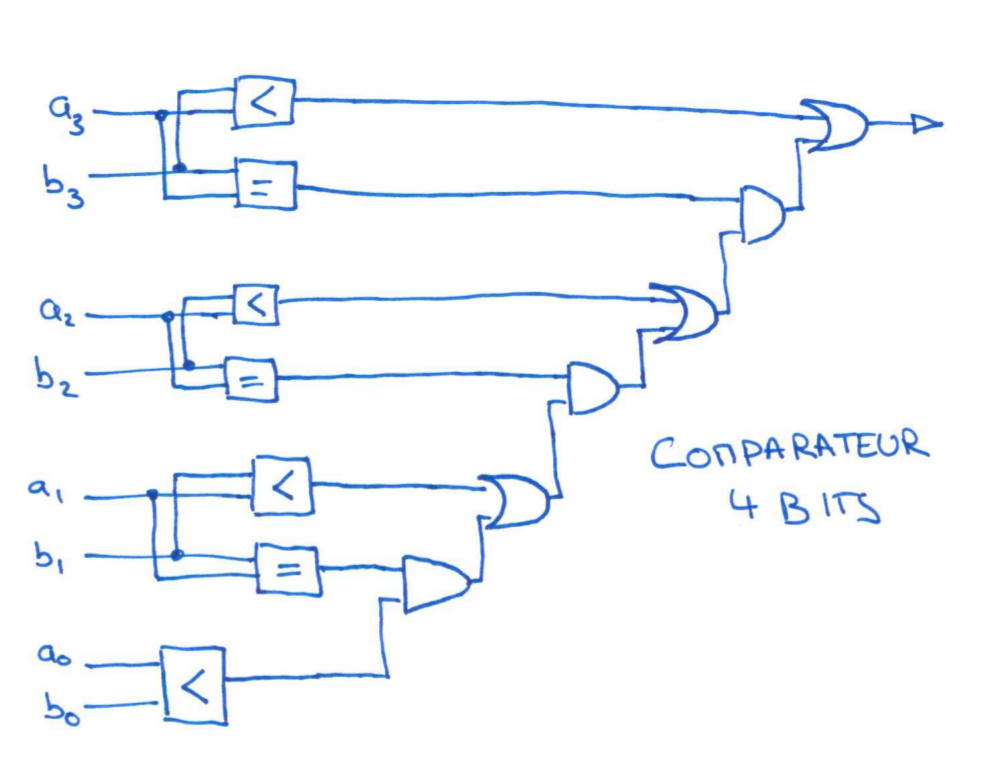
\includegraphics[width=6cm]{comparateur-msb.png}

\end{solution}

\end{enumerate}

\section{Circuits additioneurs}
\begin{enumerate}
\item Un demi additionneur est composé de:
  \begin{itemize}
  \item deux entrées: les bits $a$ et $b$
  \item deux sorties: $s$ la somme des deux bits et $r$ l'éventuelle retenue.
  \end{itemize}
  Donner les expressions booléennes de $s$ et $r$ en fonction de $a$ et $b$.
\begin{solution}
  $s = a \oplus b$ et $r = ab$.
\end{solution}
\item Proposer un circuit pour le demi additionneur.
\begin{solution}
\begin{tikzpicture}[circuit logic CDH,
tiny circuit symbols,
every circuit symbol/.style={
fill=white,draw}]
\matrix[column sep=0.7cm, row sep=0.7cm]
{
\node (A) {a};  & \node [xor gate] (x) {};& \node (S) {s};  \\
\node (B) {b};  & \node [and gate] (a) {};& \node (R) {r};\\
};
\draw (A.east) -- ++(right:3mm) |- (x.input 1);
\draw (B.east) -- ++(right:6mm) |- (x.input 2);
\draw (A.east) -- ++(right:3mm) |- (a.input 1);
\draw (B.east) -- ++(right:6mm) |- (a.input 2);

\draw (x.output) -- ++(right:3mm) |- (S.west);
\draw (a.output) -- ++(right:3mm) |- (R.west);
\end{tikzpicture}
\end{solution}
\item Un additionneur complet est composé de:
  \begin{itemize}
    \item trois entrées: les bits $a$ et $b$ et $r_0$ la retenue
      propagé par l'additionneur précédent.
    \item deux sorties: $s = a + b + r_0 [2]$ et $r_1$ l'éventuelle retenue lors
      du calcul de $s$.
  \end{itemize}
  Construire un circuit pour l'additionneur complet. Pour cela utiliser
  deux demi-additionneur ainsi qu'une porte OU.

\begin{solution}
\begin{tikzpicture}[circuit logic CDH,
tiny circuit symbols,
every circuit symbol/.style={
fill=white,draw}]
\matrix[column sep=0.7cm, row sep=0.7cm]
{
\node (A) {a};  &                                                    & &&\\
                & \node[draw] (ha1) {$\frac{1}{2}+$}; & \node[draw] (ha2) {$\frac{1}{2}+$};& \node (outs) {s};&\\
\node (B) {b};  & \node (R)[yshift=3mm] {$r0$};                   &                                    &\node (o) [or gate] {}; & \node (outr) {r};\\
};
\draw (A.east) -- ++(right:3mm) |- ([yshift=1mm]ha1.west) ;
\draw (B.east) -- ++(right:6mm) |- ([yshift=-1mm]ha1.west);
\draw ([yshift=1mm]ha1.east) -- ++(right:3mm) |- ([yshift=1mm]ha2.west);
\draw (R.east) -- ++(right:6mm) |- ([yshift=-1mm]ha2.west);

\draw ([yshift=-1mm]ha1.east) -- ++(right:3mm) |- (o.input 2);
\draw ([yshift=-1mm]ha2.east) -- ++(right:3mm) |- (o.input 1);


\draw (o.output) -- (outr);
\draw (ha2.east) -- (outs);
\end{tikzpicture}
\end{solution}


\item Additionneur 4 bits. Un additionneur 4 bits possède 8 signaux en entrée et
  5 signaux en sortie:
  \begin{itemize}
    \item entrées: $A=a_3a_2a_1a_0$ et $B=b_3b_2b_1b_0$ deux nombres codés sur
      4 bits chacun.
    \item sorties: $C=c_3c_2c_1c_0$ et $r$. C est la somme de $A$ et $B$ et $r$
      l'éventuelle retenue.
  \end{itemize}
  En utilisant les circuits des questions précédentes proposer un circuit pour
  l'additionneur 4 bits.

\begin{solution}
    On met en série: demi-additionneur et trois additioneurs complets.
    La retenue se propage d'une additionneur au suivant.

    Attention le temps de calcul est limité par la propagagtion de la retenue. Pour des mots grande taille (16 bits), il vaut
    mieux utiliser des additionneurs plus complexes comme le Carry Look Ahead (CLA) addder.
\end{solution}
\end{enumerate}

\end{document}
